\documentclass[11pt]{article}

\usepackage[margin=1in]{geometry}
\usepackage{amsfonts, amsmath, amssymb}
\usepackage{fancyhdr, float, graphicx}
\usepackage[utf8]{inputenc} % Required for inputting international characters
\usepackage[T1]{fontenc} % Output font encoding for international characters
\usepackage{fouriernc} % Use the New Century Schoolbook font
\usepackage[nottoc, notlot, notlof]{tocbibind}
\usepackage{listings}
\usepackage{xcolor}
\usepackage{blindtext}
\usepackage{hyperref}
\hypersetup{
	colorlinks=true,
	linkcolor=black,
	filecolor=magenta,
	urlcolor=blue,
	pdfpagemode=FullScreen,
}

\definecolor{codegreen}{rgb}{0,0.6,0}
\definecolor{codegray}{rgb}{0.5,0.5,0.5}
\definecolor{codepurple}{rgb}{0.58,0,0.82}
\definecolor{backcolour}{rgb}{0.95,0.95,0.92}

\lstdefinestyle{mystyle}{
	backgroundcolor=\color{backcolour},
	commentstyle=\color{codegreen},
	keywordstyle=\color{magenta},
	numberstyle=\tiny\color{codegray},
	stringstyle=\color{codepurple},
	basicstyle=\ttfamily\footnotesize,
	breakatwhitespace=false,
	breaklines=true,
	captionpos=b,
	keepspaces=true,
	numbers=left,
	numbersep=5pt,
	showspaces=false,
	showstringspaces=false,
	showtabs=false,
	tabsize=2
}

\lstset{style=mystyle}

% Header and Footer
\pagestyle{fancy}
\fancyhead{}
\fancyfoot{}
\fancyhead[L]{\textit{\Large{Blockchain Technology}}}
\fancyhead[R]{\textit{Krishnaraj T}}
\fancyfoot[C]{\thepage}
\renewcommand{\footrulewidth}{1pt}

\begin{document}

\begin{titlepage}
	\centering

	%---------------------------NAMES-------------------------------

	\huge\textsc{
		MIT World Peace University
	}\\

	\vspace{0.75\baselineskip} % space after Uni Name

	\LARGE{
		Attack Research and Documentation\\
		Fourth Year B. Tech, Semester 8
	}

	\vfill % space after Sub Name

	%--------------------------TITLE-------------------------------

	\rule{\textwidth}{1.6pt}\vspace*{-\baselineskip}\vspace*{2pt}
	\rule{\textwidth}{0.6pt}
	\vspace{0.75\baselineskip} % Whitespace above the title

	\huge{\textsc{
        Solidity Programming of simple Smart Contracts
    }} \\

	\vspace{0.5\baselineskip} % Whitespace below the title
	\rule{\textwidth}{0.6pt}\vspace*{-\baselineskip}\vspace*{2.8pt}
	\rule{\textwidth}{1.6pt}

	\vspace{1\baselineskip} % Whitespace after the title block

	%--------------------------SUBTITLE --------------------------	

	\LARGE\textsc{
		Lab Assignment 2
	} % Subtitle or further description
	\vfill

	%--------------------------AUTHOR-------------------------------

	Prepared By \vspace{0.5\baselineskip} % Whitespace before the editors

	\Large{
		Krishnaraj Thadesar \\
		Cyber Security and Forensics\\
        Batch A1, PA 15
	}

	\vspace{0.5\baselineskip} % Whitespace below the editor list
	\today

\end{titlepage}

\tableofcontents
\thispagestyle{empty}
\clearpage

\setcounter{page}{1}

\section{Aim}

\section{Demo}

\begin{figure}[H]
    \centering
    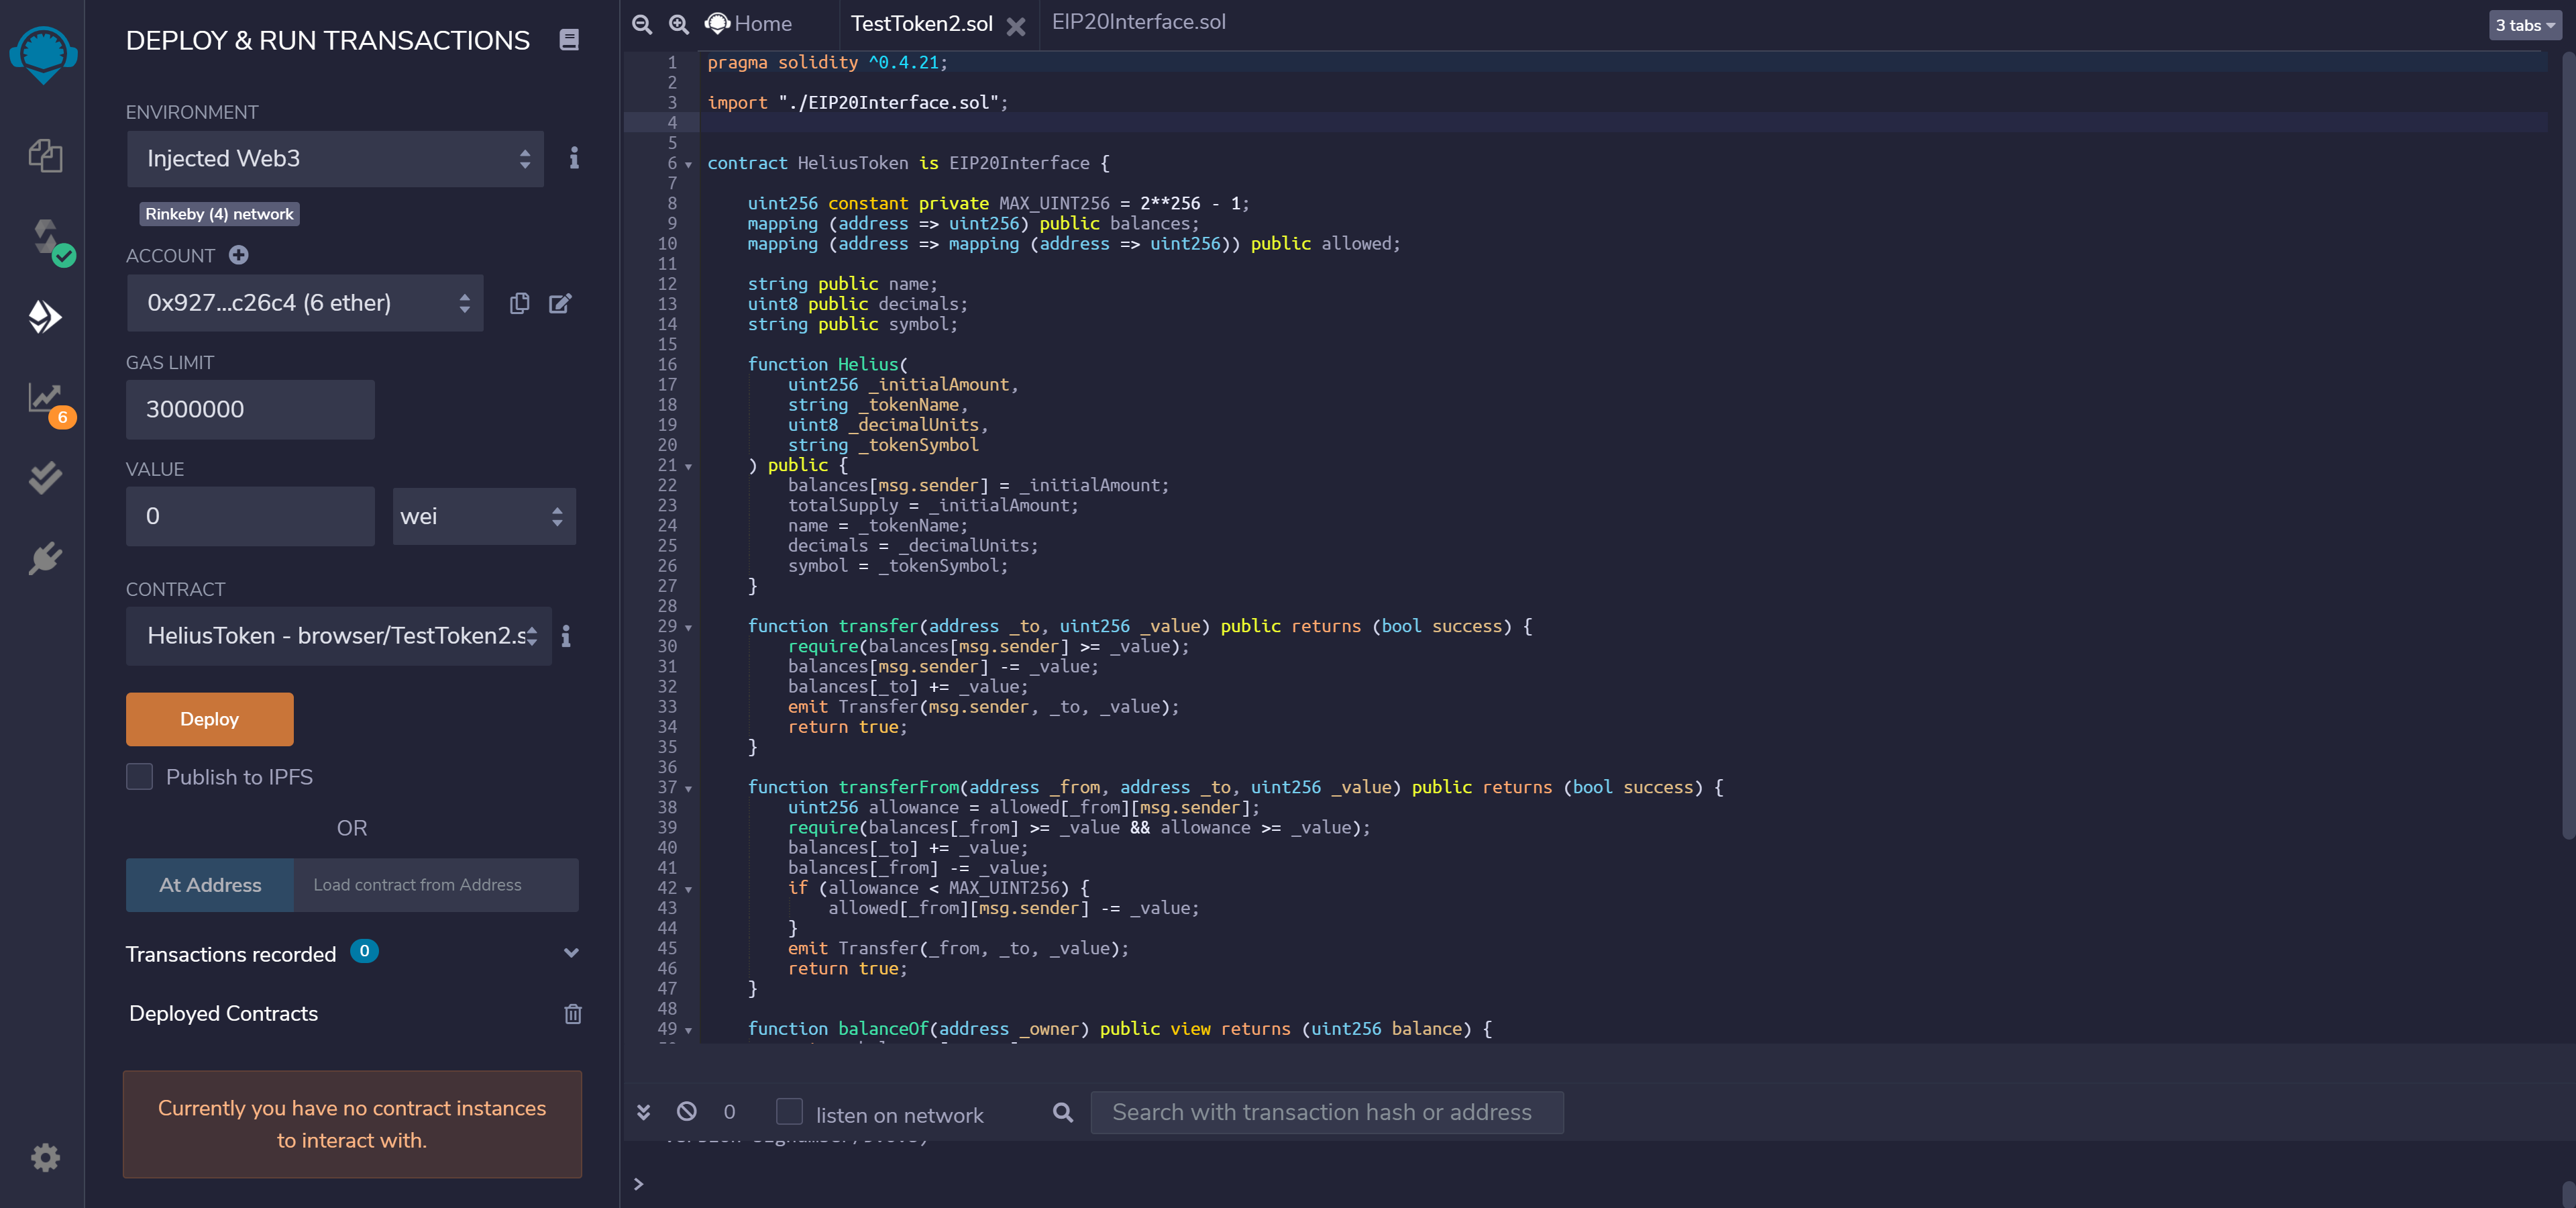
\includegraphics[width=0.8\textwidth]{dg8cf.png}
    \caption{The Remix IDE}
    \label{fig:1}
\end{figure}

\section{Frequently Asked Questions}

\subsection{What is the Concept of Gas in Solidity? How can a Developer Optimize Gas Usage in Smart Contracts?}

Gas in Solidity refers to the computational cost required to execute operations on the Ethereum Virtual Machine (EVM). Each operation consumes a certain amount of gas, and users must pay for execution in Ether. Optimizing gas usage is crucial for reducing transaction costs and improving efficiency. Developers can optimize gas usage by:

\begin{itemize}
    \item \textbf{Minimizing Storage Writes:} Using storage (e.g., \texttt{storage} variables) is expensive; prefer \texttt{memory} or \texttt{calldata} where possible.
    \item \textbf{Using Shorter Data Types:} Using \texttt{uint8} instead of \texttt{uint256} can save gas when appropriate.
    \item \textbf{Packing Storage Variables:} Grouping variables of the same type reduces storage slots used.
    \item \textbf{Avoiding Unnecessary Computation:} Precomputing values off-chain and passing them as function arguments reduces computation costs.
    \item \textbf{Using \texttt{view} and \texttt{pure} Functions:} These functions do not modify the blockchain and save gas.
\end{itemize}

\subsection{What are the Key Features of Remix IDE and How Does it Simplify the Development of Ethereum Smart Contracts?}

Remix IDE is a powerful web-based development environment for writing, testing, and deploying Solidity smart contracts. Key features include:

\begin{itemize}
    \item \textbf{Built-in Solidity Compiler:} Allows real-time compilation with error highlighting.
    \item \textbf{Debugger:} Provides step-by-step execution for debugging smart contracts.
    \item \textbf{Deployment and Interaction:} Supports deployment on local, test, and mainnet environments.
    \item \textbf{Remix Plugins:} Extensible via plugins such as Solidity Static Analysis and Gas Estimator.
    \item \textbf{Integrated Terminal:} Allows running scripts, interacting with deployed contracts, and monitoring logs.
\end{itemize}

\subsection{How Does the "Solidity Compiler" Plugin in Remix Work, and What Options Does it Provide for Developers?}

The Solidity Compiler plugin in Remix is used to compile Solidity code into bytecode that the Ethereum Virtual Machine (EVM) can execute. It provides various options for developers:

\begin{itemize}
    \item \textbf{Compiler Version Selection:} Allows choosing a specific Solidity version to ensure compatibility.
    \item \textbf{Optimization Settings:} Enables toggling optimizations to reduce gas costs.
    \item \textbf{EVM Target Selection:} Allows specifying the EVM version for backward compatibility.
    \item \textbf{Auto Compilation:} Automatically compiles the contract upon changes.
    \item \textbf{Metadata Generation:} Generates ABI (Application Binary Interface) and contract metadata.
\end{itemize}

\subsection{4. What is the Difference Between Public, Internal, and Private Visibility in Solidity?}

In Solidity, visibility modifiers determine access control for contract functions and state variables:

\begin{itemize}
    \item \textbf{Public:} Accessible from within the contract, derived contracts, and externally via transactions.
    \item \textbf{Internal:} Accessible only within the contract and its derived contracts, but not externally.
    \item \textbf{Private:} Restricted to the defining contract; not accessible from derived contracts or externally.
\end{itemize}

\section{Conclusion}

Understanding gas optimization techniques, development tools like Remix IDE, and Solidity-specific features such as compiler options and visibility modifiers is crucial for writing efficient smart contracts. Optimizing gas usage can significantly reduce transaction costs, while utilizing tools like Remix simplifies the development and debugging process. Proper use of visibility modifiers ensures security and proper contract structure, improving maintainability and reliability of Ethereum smart contracts.



% \begin{figure}[H]
%     \centering
%     \includegraphics[width=0.8\textwidth]{}
%     \caption{}
%     \label{fig:1}
% \end{figure}


\clearpage
\begin{thebibliography}{99}
    \bibitem{solidity_docs}
    Solidity Documentation. Available at: \url{https://docs.soliditylang.org/}

    \bibitem{remix_ide}
    Remix IDE Documentation. Available at: \url{https://remix-ide.readthedocs.io/}

    \bibitem{ethereum_gas}
    Ethereum Gas and Fees. Available at: \url{https://ethereum.org/en/developers/docs/gas/}

    \bibitem{solidity_optimizations}
    Solidity Optimizations. Available at: \url{https://docs.soliditylang.org/en/latest/internals/optimizations.html}

    \bibitem{solidity_visibility}
    Solidity Visibility and Accessors. Available at: \url{https://docs.soliditylang.org/en/latest/contracts.html#visibility-and-getters}
\end{thebibliography}

\end{document}